\section{Sums, Temperature and the Puzzles Revisited}\label{sec:sums}

Most endgames are sums of components. We recall two principles for playing them, apply them to three puzzles,
and ask when a sum names the same winner as the whole board.

\subsection{Two Principles}

\emph{Principle 1 (number avoidance).} In a sum of numbers and games that are not numbers, a player who can win
can do so without moving in a number~\cite{WinningWays,Siegel2013}.

\emph{Principle 2 (the hottest move).} Move in the component with the highest temperature
(Section~\ref{sec:notation}). For a switch $\game{x}{y}$ between numbers $x>y$, the temperature $(x-y)/2$ is
what each side gains by moving there first, and infinitesimals have temperature $0$. Principle~2 is a
heuristic, not a theorem, but it finds the winning move in every example below.

\subsection{The Puzzles Revisited}

\begin{figure}[!t]
\centering
\begin{subfigure}{0.32\columnwidth}\centering
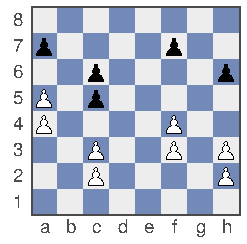
\includegraphics[width=\linewidth]{figures/puzzle71.pdf}
\caption{Puzzle 1}\label{fig:puzzle71}
\end{subfigure}\hfill
\begin{subfigure}{0.32\columnwidth}\centering
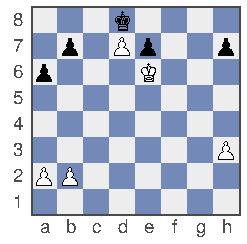
\includegraphics[width=\linewidth]{figures/puzzle72.pdf}
\caption{Puzzle 2}\label{fig:puzzle72}
\end{subfigure}\hfill
\begin{subfigure}{0.32\columnwidth}\centering
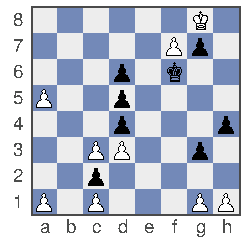
\includegraphics[width=\linewidth]{figures/puzzle73.pdf}
\caption{Puzzle 3}\label{fig:puzzle73}
\end{subfigure}
\caption{The three puzzles of~\cite{Study2025} (cylinder: files a and h adjacent); Table~\ref{tab:puzzles}
gives their exact values. (a)~White wins whoever moves first. (b)~The pawn part is an infinitesimal.
(c)~Puzzle~3 as first drawn: $+\BIG$ (not legal).}
\label{fig:puzzles}
\end{figure}


Fig.~\ref{fig:puzzles} shows three puzzles on the cylinder, and Table~\ref{tab:puzzles} compares the values
first claimed for them~\cite{Study2025} with the exact ones; the earlier walk-throughs pick the right
winners, but not always the right values.

\begin{table}[!t]
\centering
\caption{Puzzles of Fig.~\ref{fig:puzzles}: Claimed and Exact Values \lab{C2}}
\label{tab:puzzles}
\begin{tabular}{@{}lll@{}}
\toprule
Part & Claimed~\cite{Study2025} & Exact \\
\midrule
1: c-file & $\pm1$ & $\pm1$ \\
1: f-file & $\game{\game{2}{1}}{0}$ & the same (mean $3/4$) \\
1: files h, a & $1$ & $\game{+\BIG}{\star}$ (hot) \\
1: total & $1\pm1+\game{\game{2}{1}}{0}$ & white wins either way \\
2: pawns & $\pm1$ & infinitesimal, mean $0$ \\
2: kings & $0$ & not a zugzwang \\
3: files c, d & $1$ & $\tinyg{1}$ \\
3: total & $2$ & $+\BIG$ before any move \\
\bottomrule
\end{tabular}
\end{table}

\emph{Puzzle 1} (Fig.~\ref{fig:puzzle71}) has three components. The earlier values of the c-file, $\pm1$, and of
the f-file, $\game{\game{2}{1}}{0}$ with mean $3/4$, are right. Files h and a are not. White's a5--a6 still wins
outright, but black, moving first, plays h6$\times$a5 across the seam and leaves $\star$, not a loss, so this
part is $\game{+\BIG}{\star}$, hot, not the number $1$. The total is still a white win whoever moves first, but
play now starts in the h/a component, by far the hottest (Principle~2). White to move plays a5--a6 and wins.
Black to move does best to take on a5 at once, since every other move lets white force a passed pawn (after
h6--h5, for example, a4$\times$h5); white then plays c3--c4 in the next hottest component, and
$1+\star+\game{\game{2}{1}}{0}$ is a white win whoever moves next.

\emph{Puzzle 2} (Fig.~\ref{fig:puzzle72}) has one pawn component, on files h, a and b. The earlier walk-through
finds the right first moves, h3--h4 and a6--a5, and the right outcome, a first-player win. But the value is an
infinitesimal with mean $0$, not $\pm1$, so by Principle~2 it waits until every hot component is settled.
Its king group (Fig.~\ref{fig:kinggroup72}) is not a tr\'ebuchet either. With black to move, the d7 pawn covers
c8 and e8, so Kc7 is forced, and white takes e7 and promotes. With white to move, Kd5, Ke5 and Kf5 all draw:
black wins the d7 pawn, but the white king blockades the e-pawn. The group is a zugzwang for black only, on the
ordinary board \lab{C2} (our solver and the Lichess tablebase) and on the cylinder \lab{C1}, so the real result
of this ten-man position is open.

\emph{Puzzle 3} (Fig.~\ref{fig:puzzle73}) is illegal, with four white pawns on the first rank, and as drawn it
is decided at once, since the pawns on a5 and f7 are passed. On files c and d, white's best move, c3$\times$d4,
leaves $0$. Black's only move, d4$\times$c3, leaves $\game{0}{-1}$: white locks the files with d3--d4, while
black's d5--d4 keeps the spare move d6--d5. Thus $G=\ggame{0}{0\mid -1}=\tinyg{1}$, not $1$, and the legal copy
one rank up, \pos{W c2 c4 d4 / B c3 d5 d6 d7}, has the same value.

\subsection{When Is the Sum Model Right?}\label{sec:sums-hss}

In chess the first passed pawn ends the game; in a sum, a component with a passed pawn becomes $\pm\BIG$ and
play goes on elsewhere, so a $+\BIG$ can cancel a $-\BIG$. In $\game{\BIG}{0}+\game{0}{-\BIG}$ the first player
makes a passed pawn and wins the chess game, but the sum is $0$ for every $\BIG$, since the second player
answers in the other component \lab{P}. We write $S(X)$ for the sum model of a pawn position $X$ and $W(X)$ for
the whole-board game, which ends at the first passed pawn.

\begin{definition}[Hereditary sum safety]\label{def:hss}
A component carries a \emph{threat} for a side if a position reachable from it gives that side a passed pawn. A
position $X$ is \emph{hereditarily sum-safe} (HSS) if no position reachable from $X$ by moves of either side,
in any order, before the first passed pawn, $X$ included, has two components with threats for opposite sides.
\end{definition}

\begin{theorem}[Sum safety; \lab{AI}]\label{thm:hss}
Suppose that $X$ is HSS, that no position reachable from $X$ with two or more components has a usable en
passant right (condition (E)), and that $\BIG$ exceeds the number of moves either side can make. Then $S(X)$ and $W(X)$ have the same
outcome.
\end{theorem}

\begin{proof}[Proof sketch]
The models differ only after a passed pawn appears, say for white. By HSS no other component can then give black
one, so in the sum black runs out of moves before white's $+\BIG$ does. The full proof, by induction with (E),
is in the repository.
\end{proof}

In a random sample of $1{,}500$ positions, all $1{,}297$ HSS ones agree \lab{C1}, and with $\BIG=256$ the move
bound always holds on boards with eight ranks. HSS cannot be dropped (Proposition~\ref{prop:sumcounter});
without (E) the decomposition already fails in the pure pawn game (Proposition~\ref{prop:condE}).

\begin{proposition}[\lab{C2}]\label{prop:sumcounter}
A test of the top-level components alone is not enough: on $\cyl{8}$ with en passant off, $X=$\,\pos{W b2 d4 g3
h5 / B a7 c7 f7 g4} is a single component, spanning files f to d across the seam, so such a test passes it; yet
$S(X)$ is a black win whoever starts, while $W(X)$ is a first-player win.
\end{proposition}

Components with opposite threats appear only later in its tree, so $X$ is not HSS.

\begin{proposition}[\lab{C1}]\label{prop:condE}
In the pure pawn game, without the passed-pawn rule (play goes on until a side has no move), (E) cannot
be dropped: the sum can be wrong, even in outcome. On the ordinary board with six files and six ranks take
\pos{W a4 f4 / B b4 e5}, where black may take b4$\times$a3 en passant, since white has just played a2--a4. The
whole board is $\game{0}{-4,\,-3\pm2}$, a first-player win, while the sum of its two components is
$\game{-1\star}{-5\star}$, a black win: in the sum the en passant right survives moves in the other component. The two differ
with white to move, the case that arises inside larger sums; with black to move, as in the chess position,
both say black wins.
\end{proposition}

\emph{Two models.} Our CGT engine adds up components, as Elkies does~\cite{Elkies1996}; the independent
whole-board solver ends the game at the first passed pawn. Wherever the two disagree, in every case we tested,
our engine with splitting switched off matches the whole-board solver. The two models agree on every headline value: the $1/8$ and $\upsec\star$
positions of Section~\ref{sec:targets} in all nine settings (Section~\ref{sec:ep}), and the seven-pawn $\nim{2}$
of Section~\ref{sec:star2} in the default setting. Elsewhere they can differ, even in outcome: under the
opponent rule with the e.p.-aware test, \pos{W a3 b3 c2 e2 / B a6 c5 d5 e3} (the first five-file $\nim{2}$ of
Section~\ref{sec:star2-five}) is ${\Uparrow}$ as a sum but $\nim{2}$ on the whole board. Where they differ, we name the model we mean.
